\documentclass[a4paper,zihao=5]{ctexart}

% ---- 字体设置 ----
\setmainfont{Times New Roman}
\setsansfont{Arial}
\setmonofont{Consolas}[Scale=0.85]

% ---- 页面布局 ----
\usepackage[top=2.5cm,bottom=2.5cm,left=2.5cm,right=2.5cm]{geometry}

% ---- 数学 ----
\usepackage{amsmath,amssymb}

% ---- 图片 ----
\usepackage{graphicx}
\usepackage{float}
\usepackage{subcaption}

% ---- 代码 ----
\usepackage{listings}
\usepackage{xcolor}
\lstset{
language=C++,
basicstyle=\small\ttfamily,
keywordstyle=\color{blue}\bfseries,
commentstyle=\color{green!50!black},
stringstyle=\color{red!70!black},
numbers=left,
numberstyle=\tiny\color{gray},
numbersep=5pt,
breaklines=true,
frame=single,
tabsize=4,
showstringspaces=false
}

% ---- 其他 ----
\usepackage{booktabs}
\usepackage{enumitem}

\title{\LARGE\textbf{实验二：灰度图像的直方图规定化处理}}
\author{姓名：梁信、高居博、赵夕涵、刘嘉乐、黎玥含、赵欣瑶、罗雅丹、蓝浩宇}
\date{}

\begin{document}
\maketitle

%=====================================================
\section{实验目标}
%=====================================================

本实验的目标是掌握灰度图像的直方图处理方法，具体包括：

\begin{enumerate}[itemsep=2pt]
  \item 理解直方图均衡化（Histogram Equalization）的原理与实现；
  \item 理解直方图规定化（Histogram Specification / Matching）的原理与实现；
  \item 以正弦函数 $y = \sin(x),\ x\in[0,\pi]$ 作为目标直方图，对给定灰度图像进行规定化处理；
  \item 通过编程实现上述算法，并对处理结果进行分析。
\end{enumerate}

%=====================================================
\section{方法描述}
%=====================================================

\subsection{直方图与归一化直方图}

设灰度图像的灰度级范围为 $[0, L-1]$（本实验中 $L=256$），图像共有 $N$ 个像素。
灰度级 $k$ 出现的次数为 $n_k$，则归一化直方图（概率密度函数的离散近似）为：
\begin{equation}
  H(k) = p(r_k) = \frac{n_k}{N}, \quad k = 0, 1, \ldots, L-1
\end{equation}

\subsection{直方图均衡化}

直方图均衡化的目标是将原图直方图变换为近似均匀分布。其变换函数基于累积分布函数（CDF）：
\begin{equation}
  T_{\mathrm{se}}(k) = \mathrm{round}\!\left( (L-1) \sum_{i=0}^{k} H_s(i) \right)
  = \mathrm{round}\!\left( 255 \sum_{i=0}^{k} H_s(i) \right)
\end{equation}

其中 $H_s$ 为原图直方图。对原图每个像素灰度值 $r$ 施加变换 $s = T_{\mathrm{se}}(r)$ 即可得到均衡化图像 $I_{se}$。

\subsection{目标直方图生成}

本实验给定目标直方图为正弦函数形状：
\begin{equation}
  H_{\mathrm{dd}}'(k) = \sin\!\left(\frac{k}{255}\cdot\pi\right), \quad k = 0, 1, \ldots, 255
\end{equation}

归一化后得到目标概率分布：
\begin{equation}
  H_{\mathrm{dd}}(k) = \frac{H_{\mathrm{dd}}'(k)}{\displaystyle\sum_{i=0}^{255} H_{\mathrm{dd}}'(i)}
\end{equation}

\subsection{直方图规定化（SML单映射法）}

直方图规定化的核心思想是：通过均衡化作为"桥梁"，将原图的灰度分布映射到目标分布。具体步骤如下：

\textbf{步骤1}：计算原图直方图 $H_s$ 的均衡化变换函数：
\begin{equation}
  T_s(k) = \mathrm{round}\!\left( 255 \sum_{i=0}^{k} H_s(i) \right)
\end{equation}

\textbf{步骤2}：计算目标直方图 $H_{\mathrm{dd}}$ 的均衡化变换函数：
\begin{equation}
  G(k) = \mathrm{round}\!\left( 255 \sum_{i=0}^{k} H_{\mathrm{dd}}(i) \right)
\end{equation}

\textbf{步骤3}：对原图每个灰度级 $k$，在目标CDF映射中查找最近匹配：
\begin{equation}
  T_d(k) = \arg\min_{j \in [0,255]} \left| T_s(k) - G(j) \right|
\end{equation}

\textbf{步骤4}：对原图每个像素灰度值 $r$ 施加变换 $s = T_d(r)$，得到规定化目标图像 $I_d$。

%=====================================================
\section{实验结果}
%=====================================================

\subsection{原始图像与处理结果}

\begin{figure}[H]
  \centering
  \begin{subfigure}[b]{0.30\textwidth}
    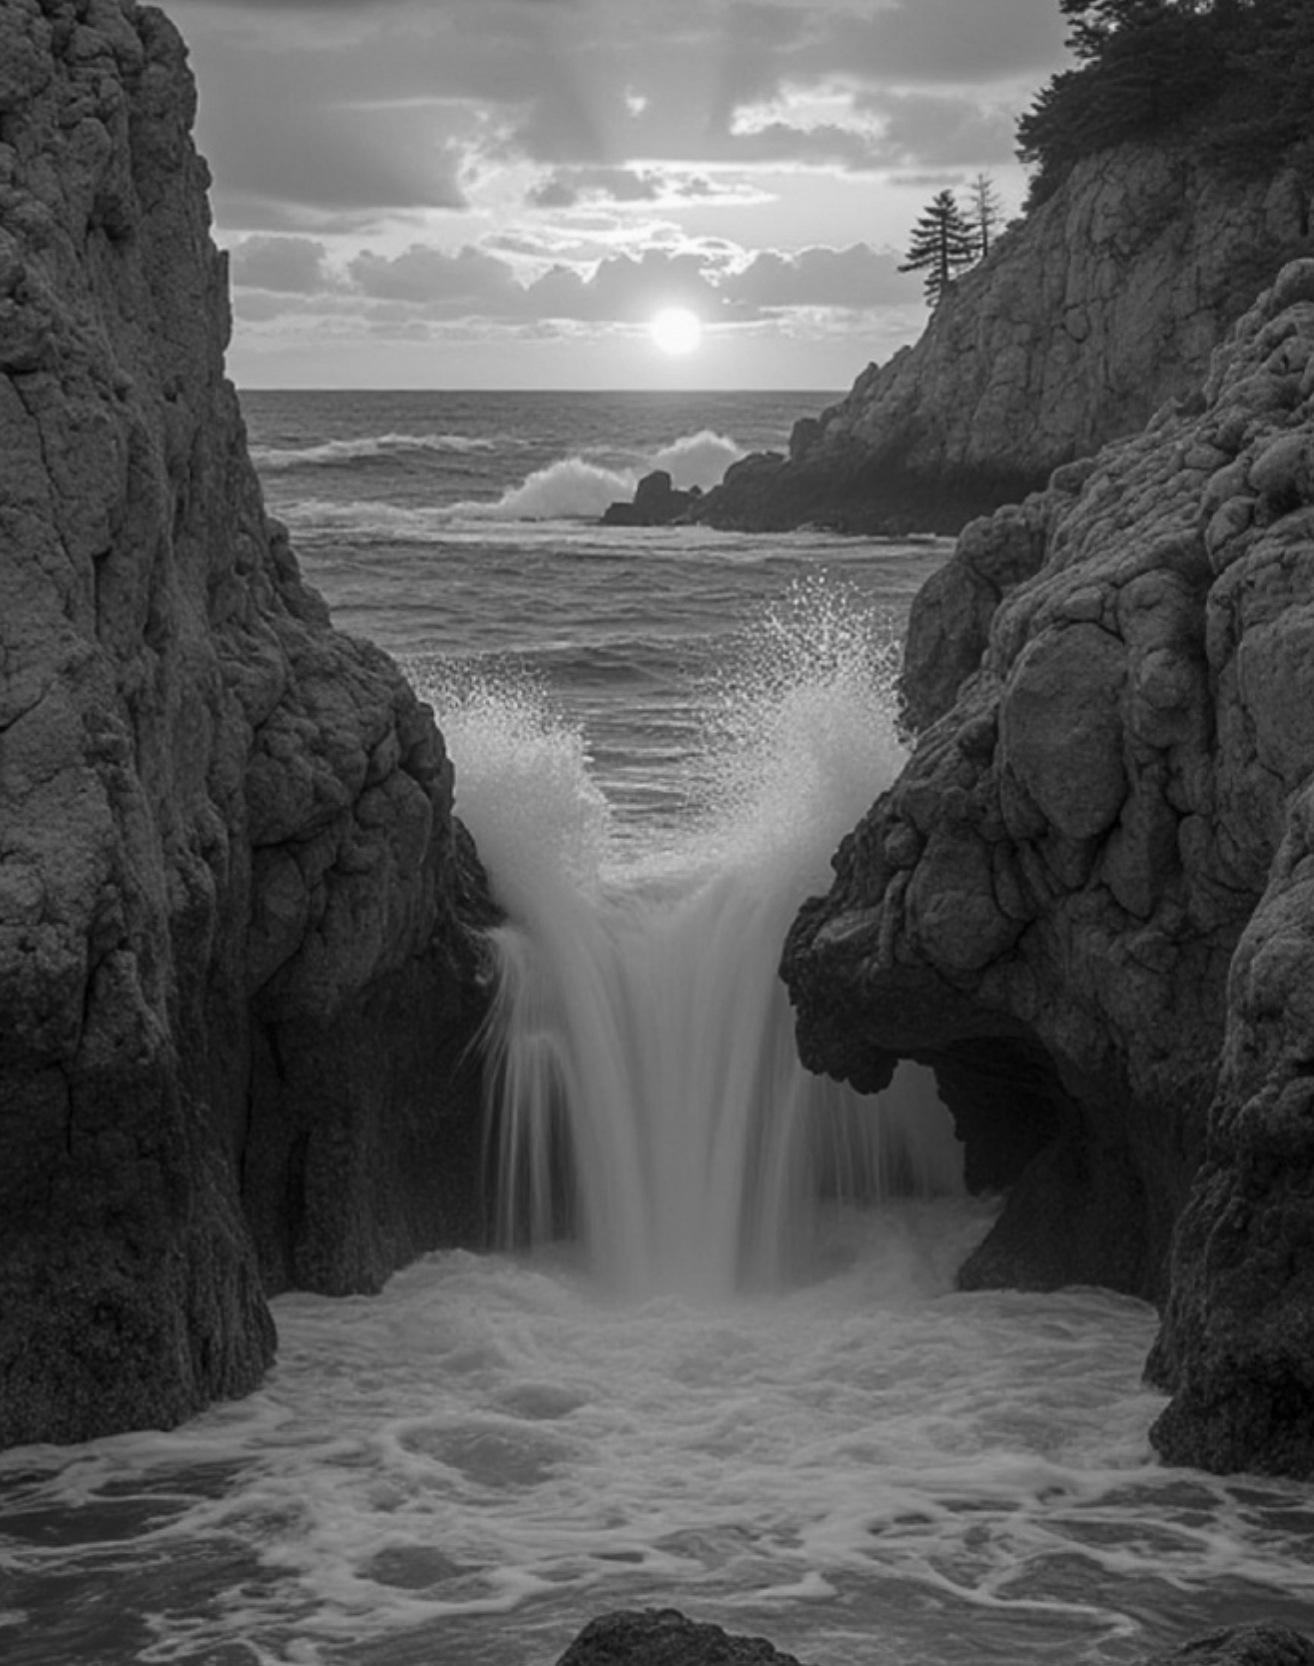
\includegraphics[width=\textwidth]{b8gray.png}
    \caption{原图 $I_s$}
  \end{subfigure}
  \hfill
  \begin{subfigure}[b]{0.30\textwidth}
    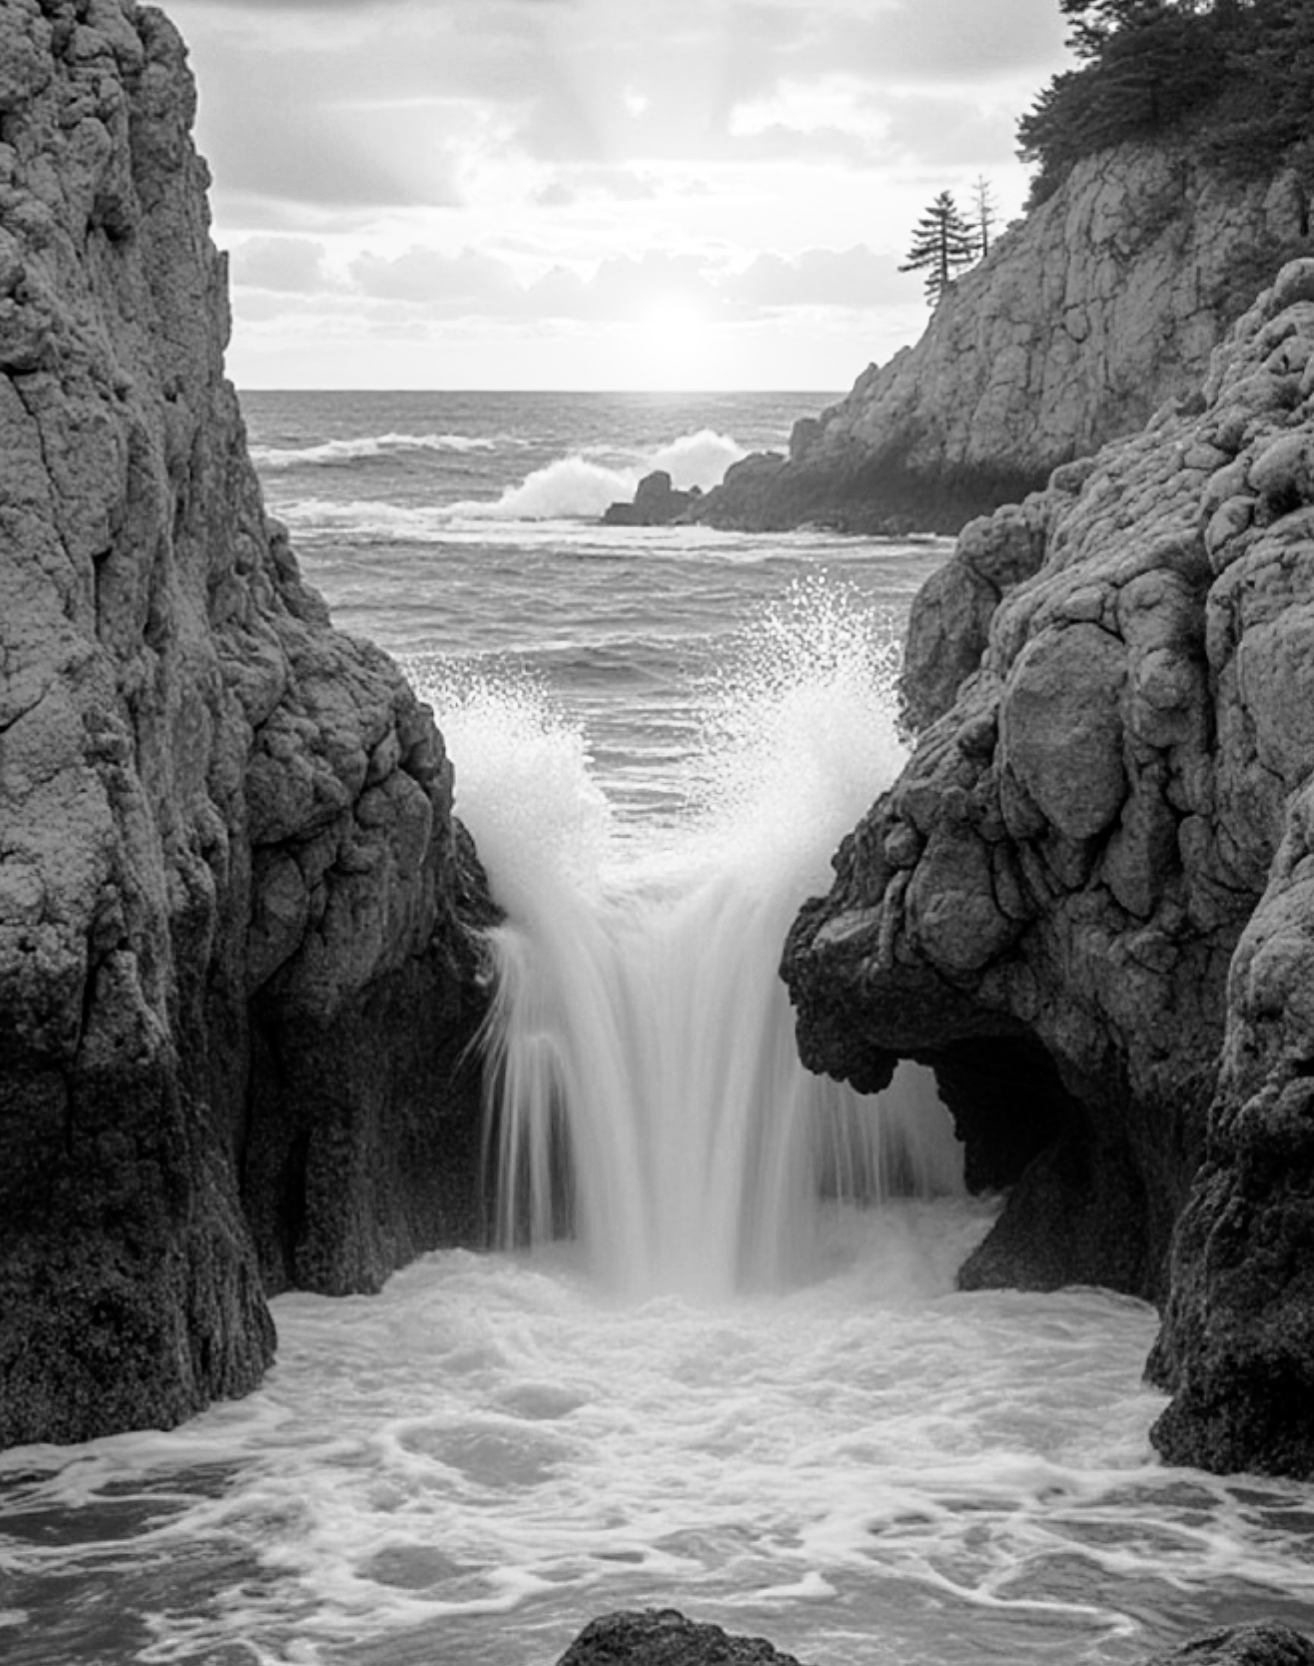
\includegraphics[width=\textwidth]{Ise.png}
    \caption{均衡化图像 $I_{se}$}
  \end{subfigure}
  \hfill
  \begin{subfigure}[b]{0.30\textwidth}
    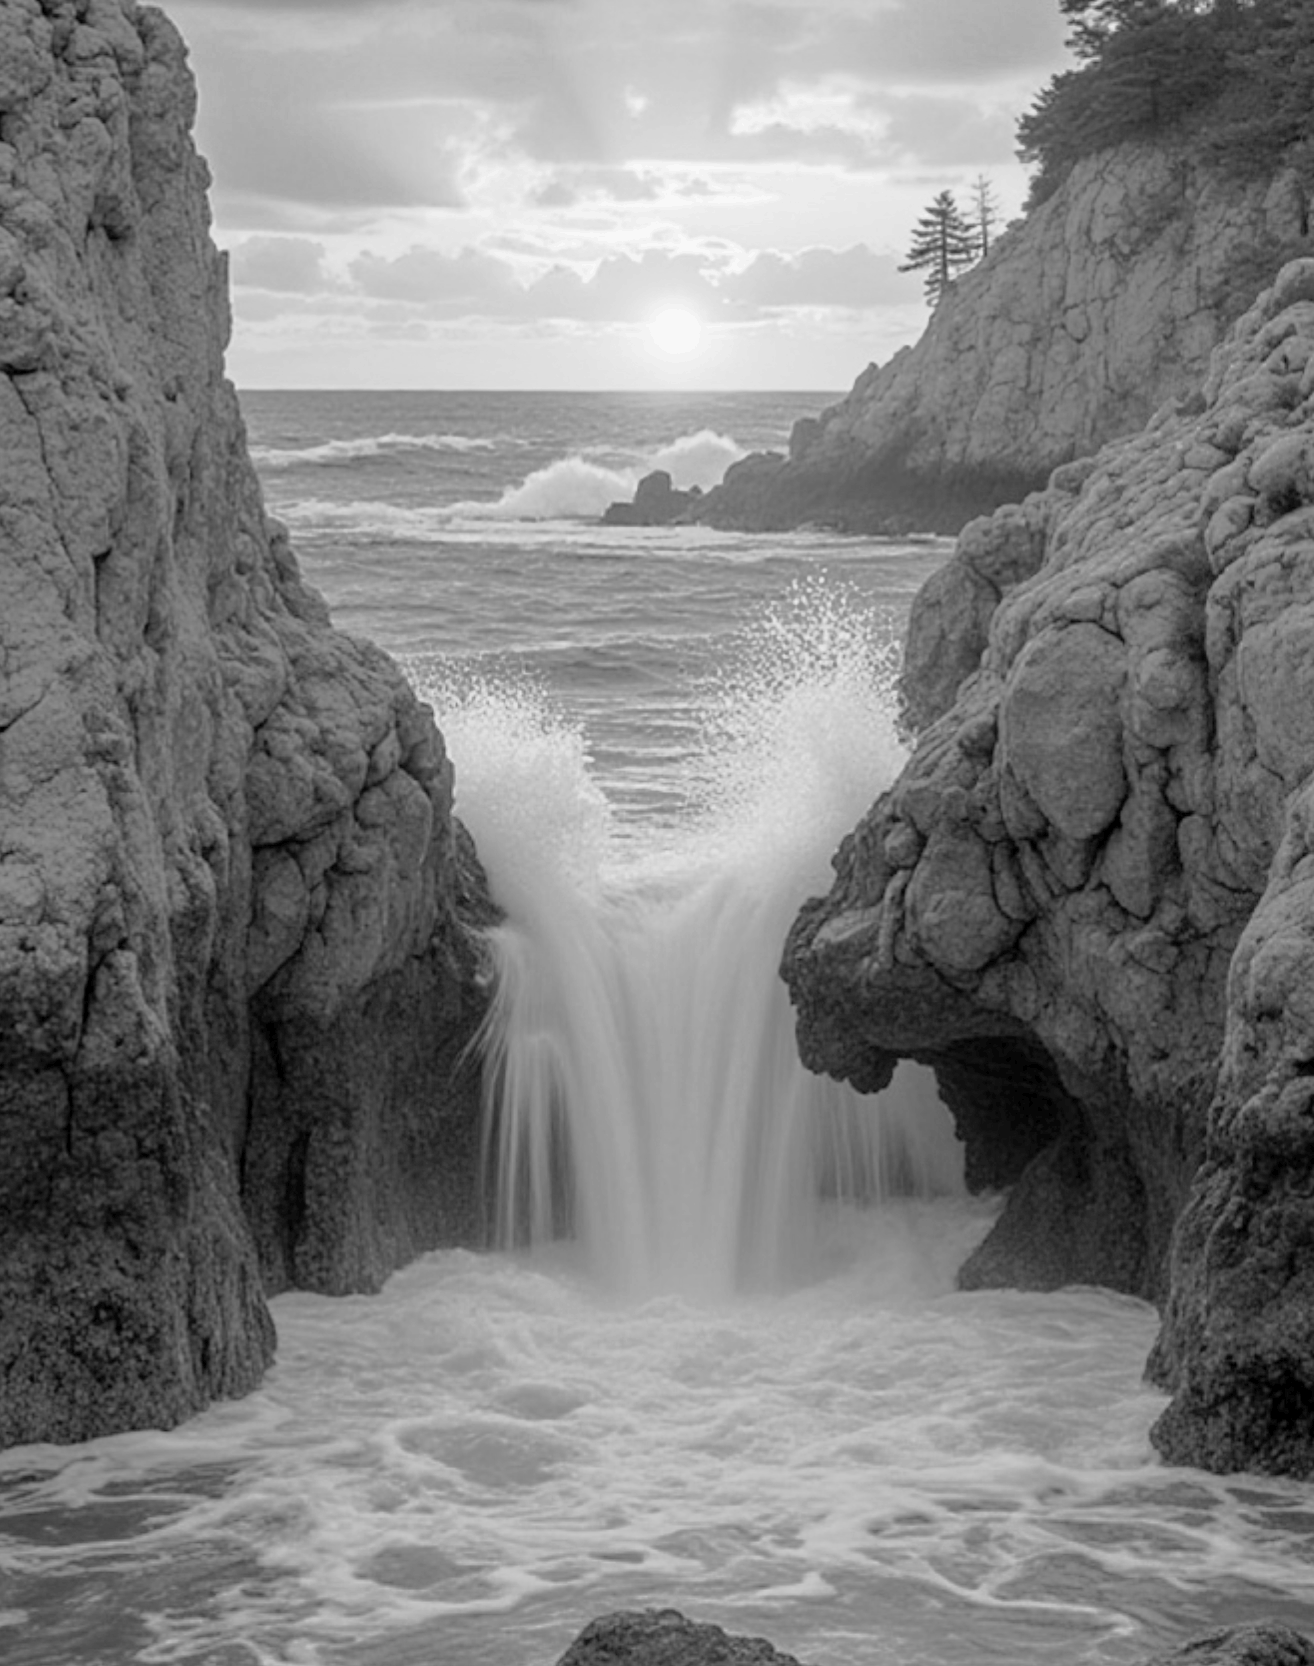
\includegraphics[width=\textwidth]{d.png}
    \caption{规定化图像 $I_d$}
  \end{subfigure}
  \caption{原始图像与处理结果对比}
\end{figure}

\subsection{任务3：原图直方图 $H_s$}

\begin{figure}[H]
  \centering
  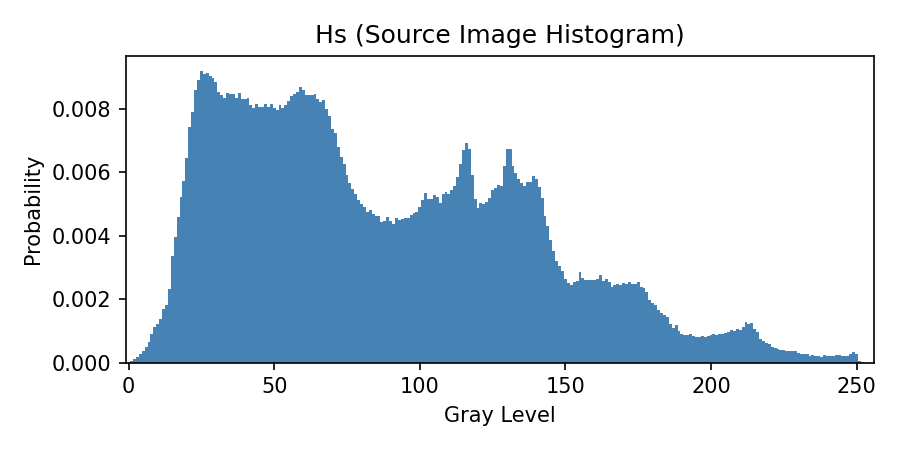
\includegraphics[width=0.85\textwidth]{fig_Hs.png}
  \caption{原图直方图 $H_s$}
\end{figure}

从图中可以看出，原图灰度值集中在中低灰度区间（约20--140），说明原图整体偏暗，对比度较低。

\subsection{任务5：均衡化变换函数 $T_{se}$}

\begin{figure}[H]
  \centering
  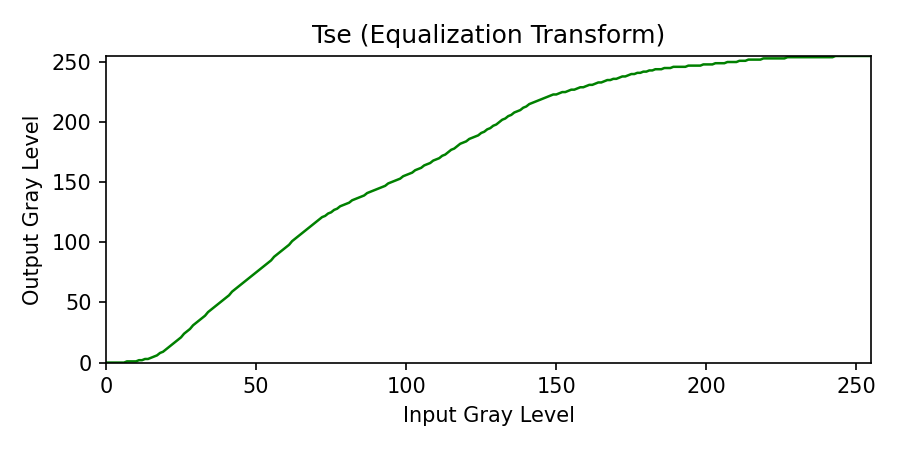
\includegraphics[width=0.85\textwidth]{fig_Tse.png}
  \caption{均衡化变换函数 $T_{se}$}
\end{figure}

均衡化变换函数为CDF的缩放映射，呈单调递增的S形曲线。在原图直方图密集的区域斜率较大（拉伸），稀疏区域斜率较小（压缩）。

\subsection{任务6：均衡化图像直方图 $H_{se}$}

\begin{figure}[H]
  \centering
  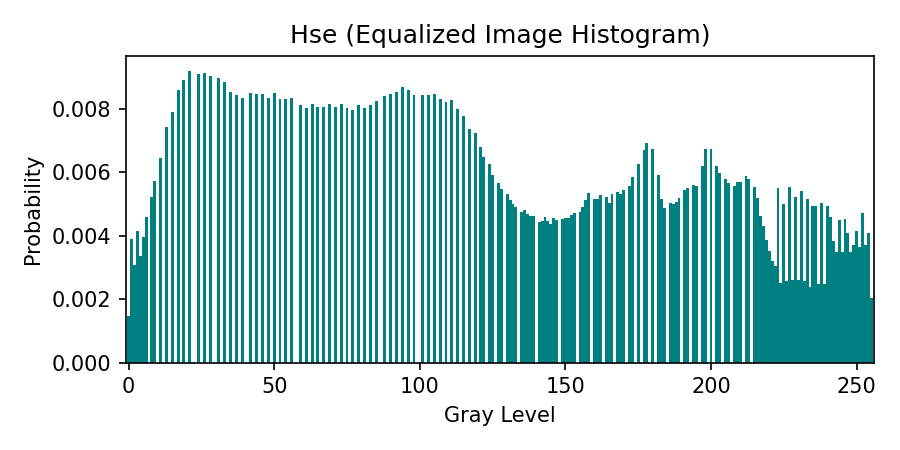
\includegraphics[width=0.85\textwidth]{fig_Hse.png}
  \caption{均衡化图像直方图 $H_{se}$}
\end{figure}

均衡化后的直方图在整个灰度范围 $[0,255]$ 上近似均匀分布，验证了均衡化算法的正确性。由于离散灰度级的限制，分布不是严格均匀的。

\subsection{目标直方图 $H_{dd}$（正弦函数）}

\begin{figure}[H]
  \centering
  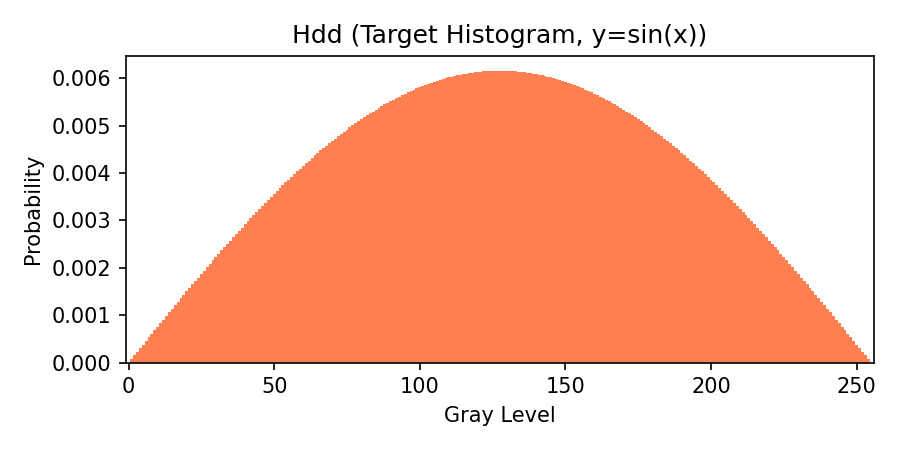
\includegraphics[width=0.85\textwidth]{fig_Hdd.png}
  \caption{目标直方图 $H_{dd}$（$y=\sin(x), x\in[0,\pi]$）}
\end{figure}

目标直方图呈正弦曲线形状，在中间灰度级（$k=128$ 附近）概率最大，两端趋近于零。

\subsection{任务2：规定化变换函数 $T_d$}

\begin{figure}[H]
  \centering
  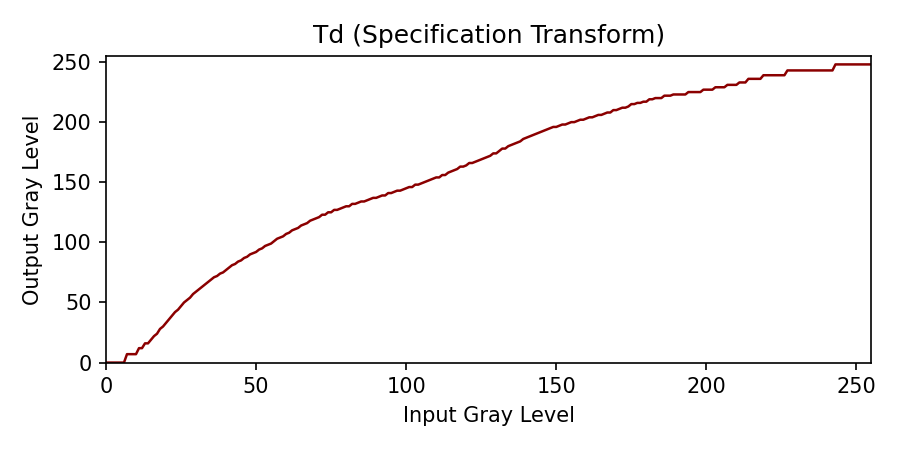
\includegraphics[width=0.85\textwidth]{fig_Td.png}
  \caption{规定化变换函数 $T_d$}
\end{figure}

规定化变换函数通过SML单映射法得到。可以看出在中间灰度区域映射较为线性，而在高灰度区出现阶梯状跳跃，这是因为正弦目标直方图在两端概率较小，多个原始灰度级被映射到同一目标灰度级。

\subsection{任务8：规定化图像直方图 $H_d$}

\begin{figure}[H]
  \centering
  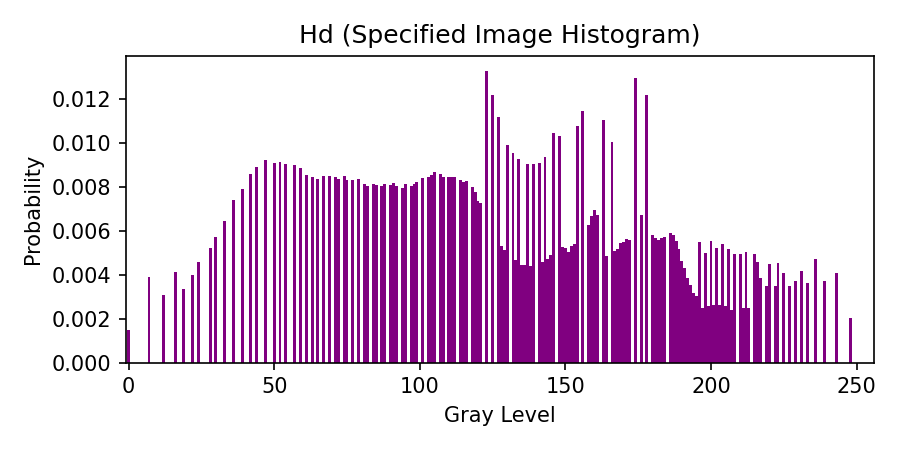
\includegraphics[width=0.85\textwidth]{fig_Hd.png}
  \caption{规定化图像直方图 $H_d$}
\end{figure}

规定化后的图像直方图整体呈现正弦函数的包络形状，中间灰度级概率较高，两端较低，与目标直方图 $H_{dd}$ 的趋势一致。由于离散映射的限制，某些灰度级概率为零（出现间隙），但整体分布已较好地逼近目标。

\subsection{任务7：规定化图像的均衡化变换函数 $T_{de}$}

\begin{figure}[H]
  \centering
  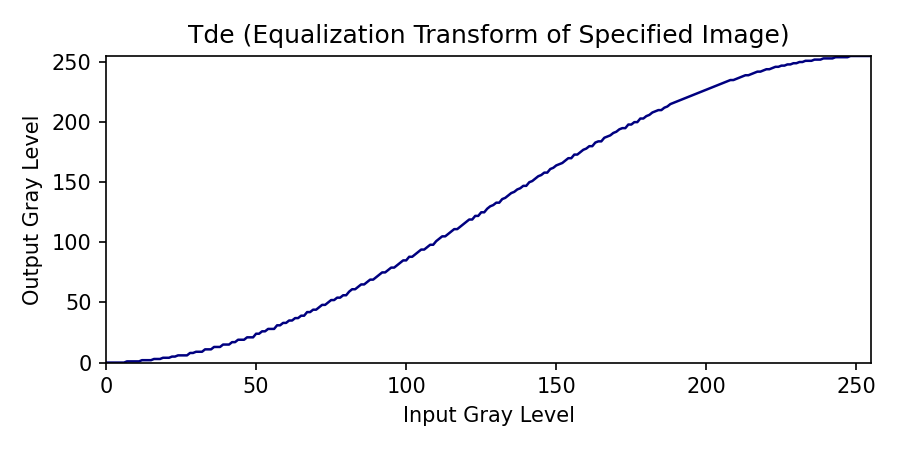
\includegraphics[width=0.85\textwidth]{fig_Tde.png}
  \caption{规定化图像的均衡化变换函数 $T_{de}$}
\end{figure}

规定化图像 $I_d$ 的均衡化变换函数呈S形曲线，与目标直方图 $H_{dd}$ 的CDF形状一致（$1-\cos(x)$ 的形态），验证了规定化处理的正确性。

\subsection{结果小结}

\begin{table}[H]
\centering
\begin{tabular}{clll}
\toprule
\textbf{任务} & \textbf{内容} & \textbf{输出文件} & \textbf{说明} \\
\midrule
1 & 规定化目标图像 $I_d$  & d.bmp      & 直方图近似正弦分布 \\
2 & 规定化变换函数 $T_d$  & Td.txt     & SML单映射法求得 \\
3 & 原图直方图 $H_s$      & Hs.txt     & 灰度集中在中低区 \\
4 & 均衡化图像 $I_{se}$   & Ise.bmp    & 对比度显著增强 \\
5 & 均衡化变换函数 $T_{se}$ & Tse.txt  & CDF缩放映射 \\
6 & 均衡化直方图 $H_{se}$ & Hse.txt    & 近似均匀分布 \\
7 & $I_d$的均衡化变换 $T_{de}$ & Tde.txt & 与目标CDF一致 \\
8 & 规定化直方图 $H_d$    & Hd.txt     & 近似正弦包络 \\
\bottomrule
\end{tabular}
\caption{实验输出文件汇总}
\end{table}

%=====================================================
\section{附录：函数代码}
%=====================================================

以下为除HXLBMPFILE类代码外的所有实现函数（main.cpp）。

\begin{lstlisting}
#include "hxlbmpfile.h"
#include <math.h>
#include <string.h>

#ifndef M_PI
#define M_PI 3.14159265358979323846
#endif

// Func1: Calc image histogram
// Input: image pointer; Output: normalized H[256]
void CalcHistogram(HXLBMPFILE* bmp, float H[256]) {
    memset(H, 0, 256 * sizeof(float));
    int total = bmp->iImageh * bmp->iImagew;
    for (int i = 0; i < bmp->iImageh; i++)
        for (int j = 0; j < bmp->iImagew; j++)
            H[bmp->pDataAt(i)[j]] += 1.0f;
    for (int k = 0; k < 256; k++)
        H[k] /= (float)total;
}

// Func2: Histogram equalization transform
// Input: normalized H; Output: mapping table T[256]
void CalcEqualizationTransform(float H[256], BYTE T[256]) {
    float cdf[256];
    cdf[0] = H[0];
    for (int i = 1; i < 256; i++)
        cdf[i] = cdf[i - 1] + H[i];
    for (int i = 0; i < 256; i++)
        T[i] = (BYTE)(cdf[i] * 255.0f + 0.5f);
}

// Func3: Generate target histogram (y=sin(x), x in [0,pi])
void GenerateTargetHistogram(float Hdd[256]) {
    float sum = 0.0f;
    for (int k = 0; k < 256; k++) {
        float x = (float)k / 255.0f * (float)M_PI;
        Hdd[k] = sinf(x);
        sum += Hdd[k];
    }
    for (int k = 0; k < 256; k++)
        Hdd[k] /= sum;
}

// Func4: Histogram specification (SML method)
void CalcSpecificationTransform(float Hs[256],
                                float Hdd[256], BYTE Td[256]) {
    BYTE Ts[256], Tdd[256];
    CalcEqualizationTransform(Hs, Ts);
    CalcEqualizationTransform(Hdd, Tdd);
    for (int k = 0; k < 256; k++) {
        int minDiff = 999, bestJ = 0;
        for (int j = 0; j < 256; j++) {
            int diff = abs((int)Ts[k] - (int)Tdd[j]);
            if (diff < minDiff) {
                minDiff = diff;
                bestJ = j;
            }
        }
        Td[k] = (BYTE)bestJ;
    }
}

// Func5: Save array to text file
void SaveArrayToTxt_Float(float arr[256],
                          const char* filename) {
    FILE* fp = fopen(filename, "w");
    if (!fp) return;
    for (int i = 0; i < 256; i++)
        fprintf(fp, "%d\t%f\n", i, arr[i]);
    fclose(fp);
}
void SaveArrayToTxt_Byte(BYTE arr[256],
                         const char* filename) {
    FILE* fp = fopen(filename, "w");
    if (!fp) return;
    for (int i = 0; i < 256; i++)
        fprintf(fp, "%d\t%d\n", i, (int)arr[i]);
    fclose(fp);
}

// Func6: Apply gray-level mapping
void ApplyTransform(HXLBMPFILE* src, BYTE T[256],
                    HXLBMPFILE* dst) {
    dst->iImagew = src->iImagew;
    dst->iImageh = src->iImageh;
    dst->iYRGBnum = 1;
    if (!dst->IspImageDataOk()) return;
    for (int k = 0; k < 256; k++) {
        dst->rgbPalette[k].rgbRed = k;
        dst->rgbPalette[k].rgbGreen = k;
        dst->rgbPalette[k].rgbBlue = k;
        dst->rgbPalette[k].rgbReserved = 0;
    }
    for (int i = 0; i < src->iImageh; i++)
        for (int j = 0; j < src->iImagew; j++)
            dst->pDataAt(i)[j] = T[src->pDataAt(i)[j]];
}

// main
int main() {
    HXLBMPFILE bmpIs;
    if (!bmpIs.LoadBMPFile((char*)"b8gray.bmp"))
        return 1;

    float Hs[256], Hdd[256], Hse[256], Hd[256];
    BYTE  Tse[256], Td[256], Tde[256];

    CalcHistogram(&bmpIs, Hs);
    SaveArrayToTxt_Float(Hs, "Hs.txt");

    CalcEqualizationTransform(Hs, Tse);
    SaveArrayToTxt_Byte(Tse, "Tse.txt");

    HXLBMPFILE bmpIse;
    ApplyTransform(&bmpIs, Tse, &bmpIse);
    bmpIse.SaveBMPFile((char*)"Ise.bmp");

    CalcHistogram(&bmpIse, Hse);
    SaveArrayToTxt_Float(Hse, "Hse.txt");

    GenerateTargetHistogram(Hdd);
    SaveArrayToTxt_Float(Hdd, "Hdd.txt");

    CalcSpecificationTransform(Hs, Hdd, Td);
    SaveArrayToTxt_Byte(Td, "Td.txt");

    HXLBMPFILE bmpId;
    ApplyTransform(&bmpIs, Td, &bmpId);
    bmpId.SaveBMPFile((char*)"d.bmp");

    CalcHistogram(&bmpId, Hd);
    SaveArrayToTxt_Float(Hd, "Hd.txt");

    CalcEqualizationTransform(Hd, Tde);
    SaveArrayToTxt_Byte(Tde, "Tde.txt");

    return 0;
}
\end{lstlisting}

\end{document}